\chapter{Imaging Excited-State Dynamics}
	The following article is a combined experimental and theoretical study focussing on imaging and characterising the dynamics following the 5p$\leftarrow$5s and 6p$\leftarrow$5s excitations of rubidium hosted by a helium nanodroplet. The experiment used femtosecond pump-probe techniques with a first laser exciting the Rb on the droplet surface at time $t_{exc}$ and a second laser ionising it for detection with VMI at time $t_{ion}$. The results characterised a critical time delay, called the ``fall-back time'', between two opposite outcomes. If $t_{ion}-t_{exc}\leq\tau$, the departing Rb atom is still rather close to the droplet when the probe laser turns their interaction to attractive. As a result, the Rb$^+$ turns around and gets solvated. On the other hand, for $t_{ion}-t_{exc}\geq\tau$, ionisation occurs too late for Rb$^+$ to feel an appreciable attraction from the droplet, and it had already too much kinetic energy, so that it escapes. 
	
	The theoretical study focussed on understanding the desorption dynamics and determining the fall-back times to compare with the experiment. It made use of the He-TDDFT presented in \scn{sec:td-dft}, both in the excited and ionised states. The results are presented in the following article which was published in the Journal of Physical Chemistry Letters\citep{Vangerow2017}.
	
	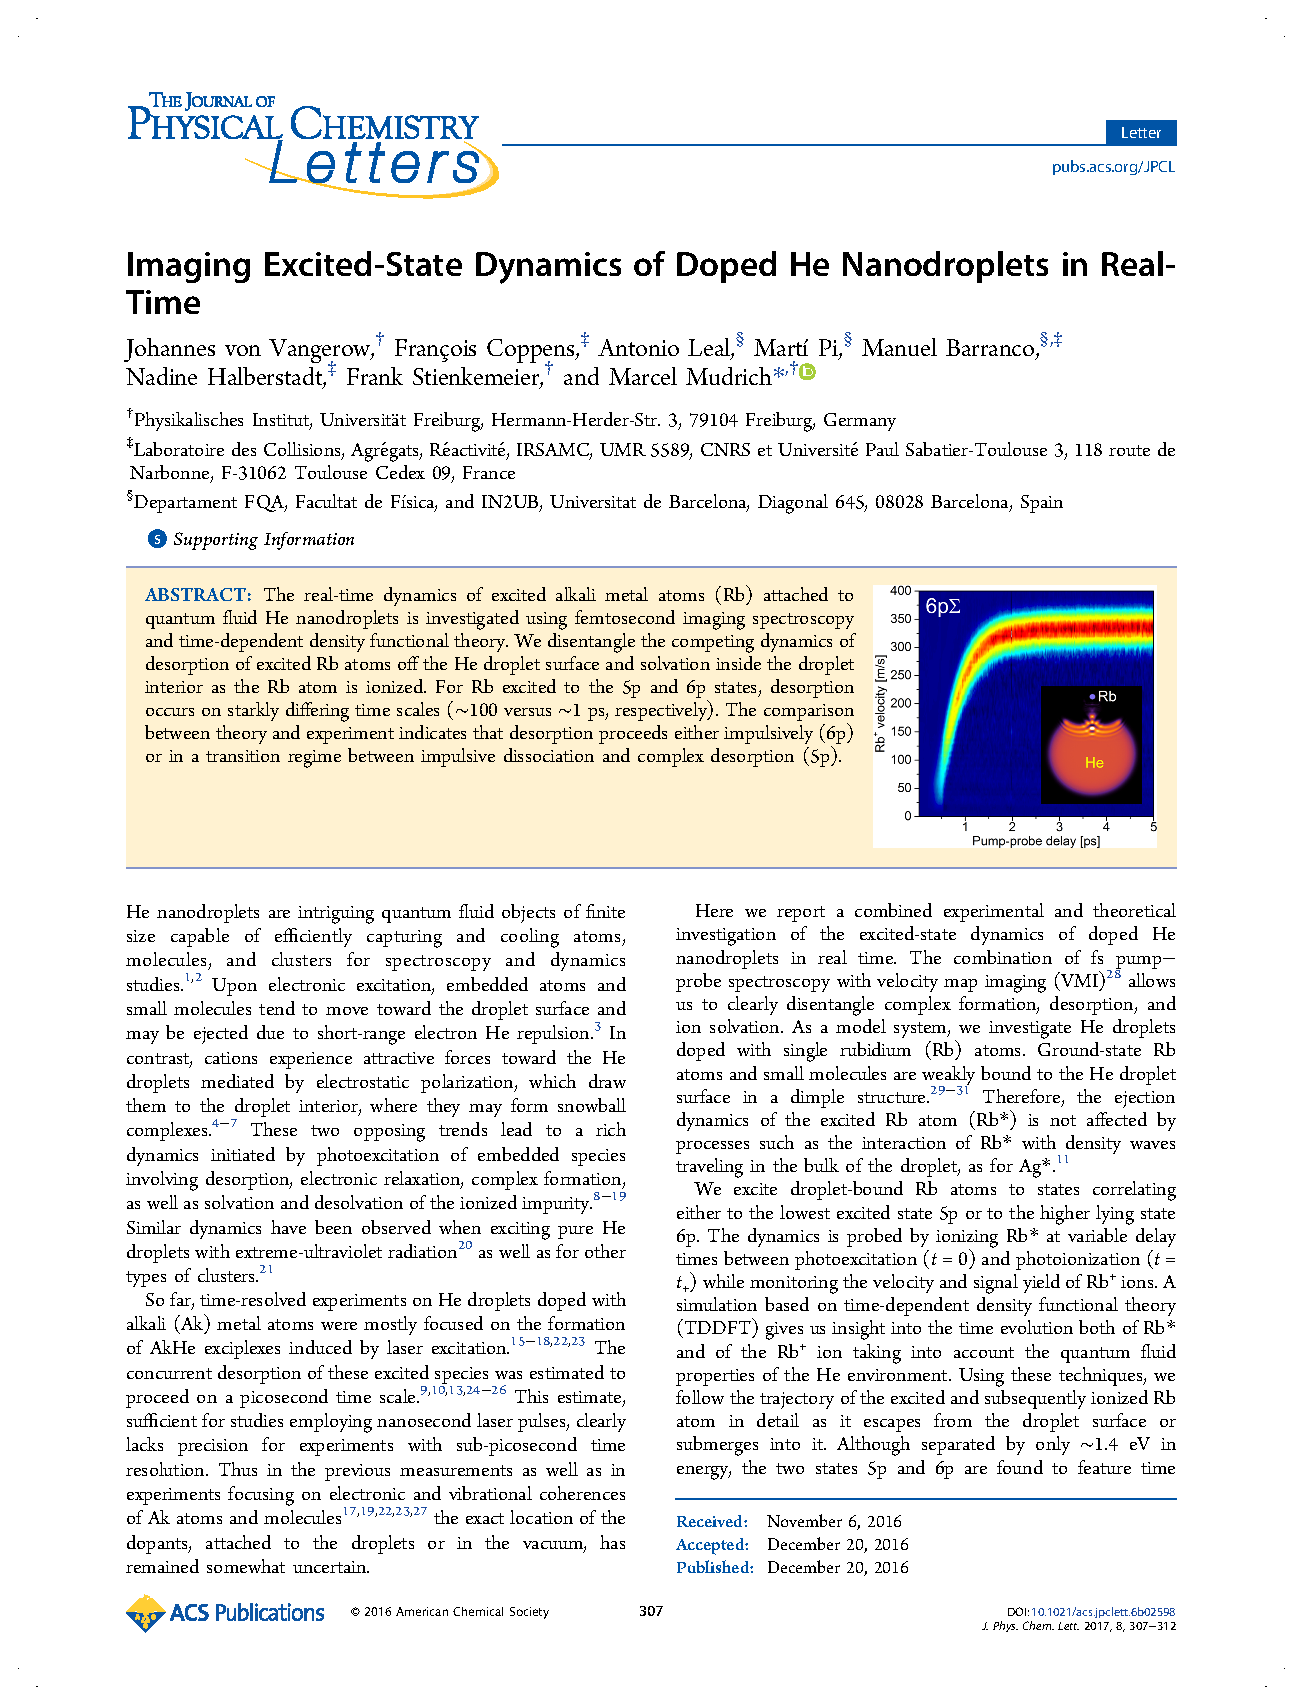
\includepdf[pages=-, scale=0.875, pagecommand={}]{jpcl_vol8_no1_pp307-312.pdf}